\documentclass[14pt,usepdftitle=false,aspectratio=169]{beamer}
\usepackage{preambule}
\setbeamercolor{structure}{fg=black}
\usepackage{tables}\usepackage{trigo}\newcommand\N{\mathbb{N}}\newcommand\R{\mathbb{R}}\let\oldlim\lim\renewcommand\lim[2]{\oldlim\limits_{#1}\l#2\r}\let\oldexp\exp\renewcommand\exp[2][]{\oldexp^{#1}\l#2\r}\let\oldln\ln\renewcommand\ln[2][]{\oldln^{#1}\l#2\r}\usepackage{graphs}\usepackage{mathtools}\usepackage{rotating}\usepackage{analyse}
\hypersetup{pdftitle=Trigonométrie 2}
\title{Trigonométrie 2}
\author{}
\date{}
\begin{document}
\begin{frame}
    \titlepage
\end{frame}
\slideq{$2\sin{x}\cos{x}$}{1/84}
\slider{$\sin{2x}$}{1/84}
\slideq{$\tan{x}$\linebreak\linebreak$t=\tan{\frac{x}{2}}$}{2/84}
\slider{$\frac{2t}{1-t^2}$\linebreak\linebreak$t=\tan{\frac{x}{2}}$}{2/84}
\slideq{Courbe représentative de $\asin{x}$}{3/84}
\slider{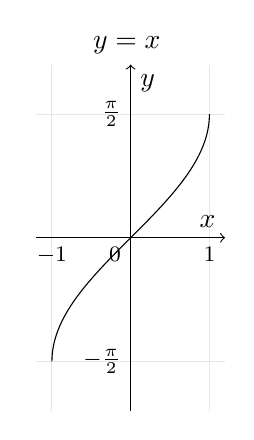
\begin{tikzpicture} \draw[color=gray,opacity=0.2] (-1.2,-2.2) grid[ystep=pi/2](1.2,2.2); \draw[->] (-1.2, 0) -- (1.2, 0) node[above left]{$x$}; \draw[->] (0,-2.2) -- (0, 2.2) node[below right]{$y$}; \foreach \y[count=\cnt] in {-\frac{\pi}{2}} \draw(0,{(-\cnt/2)*pi}) node[left]{\footnotesize$\y$}; \foreach \y[count=\cnt] in {\frac{\pi}{2}} \draw(0,{(\cnt/2)*pi}) node[left]{\footnotesize$\y$}; \foreach \x in {-1} \draw(\x,0) node[below]{\footnotesize$\x$}; \foreach \x in {1} \draw(\x,0) node[below]{\footnotesize$\x$}; \draw(0,0) node[below left]{\footnotesize$0$}; \draw[domain=-pi/2:pi/2, samples=400, scale=1, smooth, variable=\x, black] plot ({sin(\x r)},\x); \node[above] at (current bounding box.north) {$y=\asin{x}$}; \end{tikzpicture}}{3/84}
\slideq{Expression de $\ach{x}$}{4/84}
\slider{$\ln{x+\sqrt{x^2-1}}$}{4/84}
\slideq{$\sin[2]{x}$}{5/84}
\slider{$\frac{1-\cos{2x}}{2}$}{5/84}
\slideq{Courbe représentative de $\sin{x}$}{6/84}
\slider{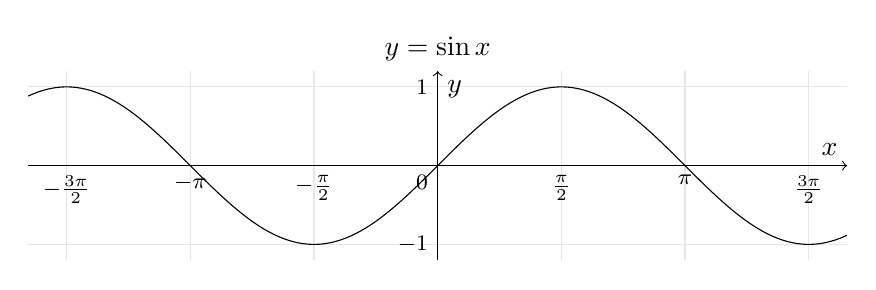
\begin{tikzpicture} \draw[color=gray,opacity=0.2] (-5.2,-1.2) grid[xstep=pi/2](5.2,1.2); \draw[->] (-5.2, 0) -- (5.2, 0) node[above left]{$x$}; \draw[->] (0,-1.2) -- (0, 1.2) node[below right]{$y$}; \foreach \y in {-1} \draw(0,\y) node[left]{\footnotesize$\y$}; \foreach \y in {1} \draw(0,\y) node[left]{\footnotesize$\y$}; \foreach \x[count=\cnt] in {-\frac{\pi}{2},-\pi,-\frac{3\pi}{2}} \draw({(-\cnt/2)*pi},0) node[below]{\footnotesize$\x$}; \foreach \x[count=\cnt] in {\frac{\pi}{2},\pi,\frac{3\pi}{2}} \draw({(\cnt/2)*pi},0) node[below]{\footnotesize$\x$}; \draw(0,0) node[below left]{\footnotesize$0$}; \draw[domain=-5.2:5.2, samples=1000, smooth, variable=\x, black] plot (\x, {sin(\x r)}); \node[above] at (current bounding box.north) {$y=\sin{x}$};\end{tikzpicture}}{6/84}
\slideq{$\lim{x\to0}{\frac{\asin{x}}{x}}$}{7/84}
\slider{$1$}{7/84}
\slideq{$\lim{x\to0}{\frac{\th{x}}{x}}$}{8/84}
\slider{$1$}{8/84}
\slideq{Courbe représentative de $\ach{x}$}{9/84}
\slider{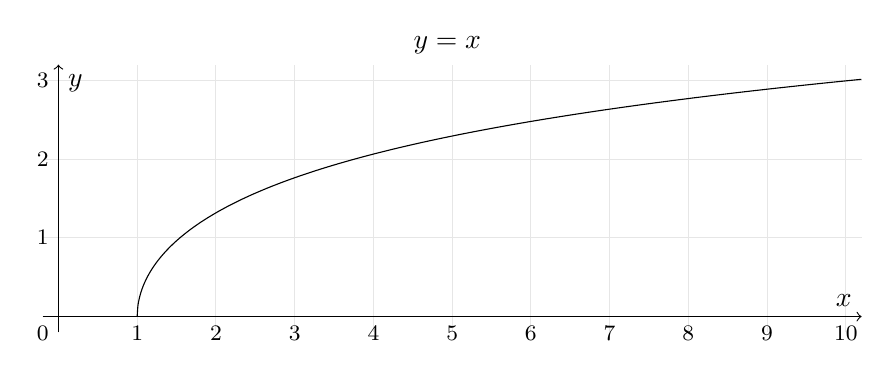
\begin{tikzpicture} \draw[color=gray,opacity=0.2] (-0.2,-0.2) grid (10.2,3.2); \draw[->] (-0.2, 0) -- (10.2, 0) node[above left]{$x$}; \draw[->] (0,-0.2) -- (0, 3.2) node[below right]{$y$}; \foreach \y in {1,...,3} \draw(0,\y) node[left]{\footnotesize$\y$}; \foreach \x in {1,...,10} \draw(\x,0) node[below]{\footnotesize$\x$}; \draw(0,0) node[below left]{\footnotesize$0$}; \draw[domain=1:10.2, samples=1100, scale=1, smooth, variable=\x, black] plot (\x,{ln(\x+sqrt(\x*\x-1))}); \node[above] at (current bounding box.north) {$y=\ach{x}$}; \end{tikzpicture}}{9/84}
\slideq{$\sin{x}\sin{y}$}{10/84}
\slider{$\frac{1}{2}\l\cos{x-y}-\cos{x+y}\r$}{10/84}
\slideq{$\lim{x\to0}{\frac{\sin{x}}{x}}$}{11/84}
\slider{1}{11/84}
\slideq{$\cot{x}$\linebreak\linebreak$t=\tan{\frac{x}{2}}$}{12/84}
\slider{$\frac{1-t^2}{2t}$\linebreak\linebreak$t=\tan{\frac{x}{2}}$}{12/84}
\slideq{$\lim{x\to0}{\frac{\tan{x}}{x}}$}{13/84}
\slider{$1$}{13/84}
\slideq{$\lim{x\to0}{\frac{\sh{x}}{x}}$}{14/84}
\slider{$1$}{14/84}
\slideq{$\sin{x}\cos{y}-\sin{y}\cos{x}$}{15/84}
\slider{$\sin{x-y}$}{15/84}
\slideq{$\sin{\pi-x}$}{16/84}
\slider{$\sin{x}$}{16/84}
\slideq{Valeurs remarquables de $\asin{x}$ et $\acos{x}$}{17/84}
\slider{\setcolrow{6}{3}\begin{tikzpicture}[ampersand replacement=\&] \matrix (mat) [table] {  \&$0$\&$\oldfrac{1}{2}$\&$\oldfrac{\sqrt{2}}{2}$\&$\oldfrac{\sqrt{3}}{2}$\&$1$\\ \begin{turn}{45}$\arcsin$\end{turn}\&$0$\&$\oldfrac{\pi}{6}$\&$\oldfrac{\pi}{4}$\&$\oldfrac{\pi}{3}$\&$\oldfrac{\pi}{2}$\\ \begin{turn}{45}$\arccos$\end{turn}\&$\oldfrac{\pi}{2}$\&$\oldfrac{\pi}{3}$\&$\oldfrac{\pi}{4}$\&$\oldfrac{\pi}{6}$\&$0$\\ }; \draw [line width=0.5mm] (-10cm/3,-6.5cm/2) -- (-10cm/3,6.5cm/2); \draw [line width=0.5mm] (-10cm/2,6.5cm/6) -- (10cm/2,6.5cm/6); \draw [line width=0.5mm] (-5cm,-3.25cm) rectangle (5cm,3.25cm); \end{tikzpicture}}{17/84}
\slideq{$\cos[2]{x}$}{18/84}
\slider{$\frac{1+\cos{2x}}{2}$}{18/84}
\slideq{$\frac{-\cot{x}\cot{y}-1}{\cot{x}-\cot{y}}=\frac{\cot{x}\cot{y}+1}{\cot{y}-\cot{x}}$}{19/84}
\slider{$\cot{x-y}$}{19/84}
\slideq{Courbe représentative de $\ath{x}$}{20/84}
\slider{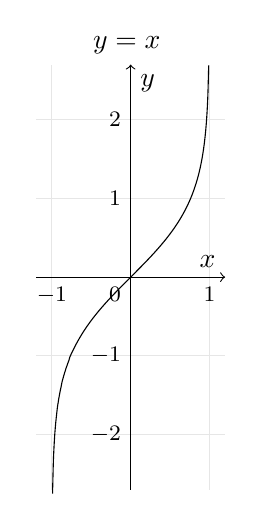
\begin{tikzpicture} \draw[color=gray,opacity=0.2] (-1.2,-2.7) grid (1.2,2.7); \draw[->] (-1.2, 0) -- (1.2, 0) node[above left]{$x$}; \draw[->] (0,-2.7) -- (0, 2.7) node[below right]{$y$}; \foreach \y in {-2,-1,1,2} \draw(0,\y) node[left]{\footnotesize$\y$}; \foreach \x in {-1} \draw(\x,0) node[below]{\footnotesize$\x$}; \foreach \x in {1} \draw(\x,0) node[below]{\footnotesize$\x$}; \draw(0,0) node[below left]{\footnotesize$0$}; \draw[domain=-0.992:0.992, samples=200, scale=1, smooth, variable=\x, black] plot (\x,{ln((1+\x)/(1-\x))/2}); \node[above] at (current bounding box.north) {$y=\ath{x}$}; \end{tikzpicture}}{20/84}
\slideq{Courbe représentative de $\atan{x}$}{21/84}
\slider{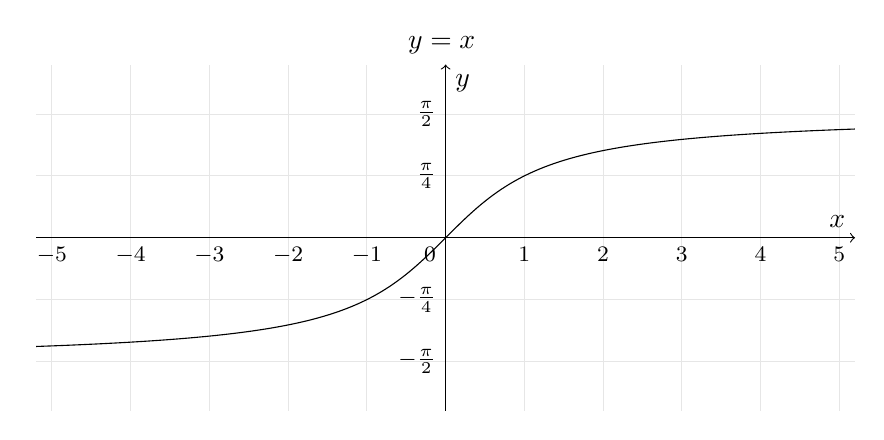
\begin{tikzpicture} \draw[color=gray,opacity=0.2] (-5.2,-2.2) grid[ystep=pi/4](5.2,2.2); \draw[->] (-5.2, 0) -- (5.2, 0) node[above left]{$x$}; \draw[->] (0,-2.2) -- (0, 2.2) node[below right]{$y$}; \foreach \y[count=\cnt] in {-\frac{\pi}{4},-\frac{\pi}{2}} \draw(0,{(-\cnt/4)*pi}) node[left]{\footnotesize$\y$}; \foreach \y[count=\cnt] in {\frac{\pi}{4},\frac{\pi}{2}} \draw(0,{(\cnt/4)*pi}) node[left]{\footnotesize$\y$}; \foreach \x in {-5,...,-1} \draw(\x,0) node[below]{\footnotesize$\x$}; \foreach \x in {1,...,5} \draw(\x,0) node[below]{\footnotesize$\x$}; \draw(0,0) node[below left]{\footnotesize$0$}; \draw[domain=-5.2:5.2, samples=2000, scale=1, smooth, variable=\x, black] plot (\x,{rad(atan(\x))}); \node[above] at (current bounding box.north) {$y=\atan{x}$}; \end{tikzpicture}}{21/84}
\slideq{$\der{\th{x}}$}{22/84}
\slider{$1-\th[2]{x}=\frac{1}{\ch[2]{x}}$}{22/84}
\slideq{$\lim{x\to0}{\frac{\ch{x}-1}{x^2}}$}{23/84}
\slider{$\frac{1}{2}$}{23/84}
\slideq{$\der{\ath{x}}$}{24/84}
\slider{$\frac{1}{1-x^2}$}{24/84}
\slideq{Propriétés remarquables de $\acos{x}$}{25/84}
\slider{$\forall x\in\left[-1,1\right],\;\cos{\acos{x}}=x$\linebreak$\forall x\in\left[0,\pi\right],\;\acos{\cos{x}}=x$\linebreak$\forall x\in\left[-\pi,0\right],\;\acos{\cos{x}}=-x$}{25/84}
\slideq{Inégalités classiques de $\sh{x}$}{26/84}
\slider{$\forall x\in\R_+,\;\sh{x}\geqslant x$\linebreak$\forall x\in\R_-,\;\sh{x}\leqslant x$}{26/84}
\slideq{$n\in\N^*$, $x\in\R$\linebreak$\der[n]{\cos{x}}$}{27/84}
\slider{$\cos{x+\frac{n\pi}{2}}=\left\{\begin{matrix*}[l]\l-1\r^{\left\lfloor\oldfrac{n}{2}\right\rfloor}\cos{x}&\;\text{si }n\in2\N\\\l-1\r^{\left\lfloor\oldfrac{n}{2}\right\rfloor+1}\sin{x}&\;\text{sinon}\end{matrix*}\right.\!$}{27/84}
\slideq{$n\in\N^*$, $x\in\R$\linebreak$\der[n]{\sh{x}}$}{28/84}
\slider{$\left\{\begin{matrix*}[l]\sh{x}&\;\text{si }n\in2\N\\\ch{x}&\;\text{sinon}\end{matrix*}\right.\!$}{28/84}
\slideq{$\sin{x+\pi}$}{29/84}
\slider{$-\sin{x}$}{29/84}
\slideq{$\cot{2x}$}{30/84}
\slider{$\frac{\cot[2]{x}-1}{2\cot{x}}$}{30/84}
\slideq{$\frac{\tan{x}+\tan{y}}{1-\tan{x}\tan{y}}$}{31/84}
\slider{$\tan{x+y}$}{31/84}
\slideq{$\der{\acos{x}}$}{32/84}
\slider{$-\frac{1}{\sqrt{1-x^2}}$}{32/84}
\slideq{Propriétés remarquables de $\atan{x}$}{33/84}
\slider{$\forall x\in\R,\;\tan{\atan{x}}=x$\linebreak$\forall x\in\left]-\oldfrac{\pi}{2},\oldfrac{\pi}{2}\right[,\;\atan{\tan{x}}=x$\linebreak$\forall n\in\N,\;\forall x\in\left]-\oldfrac{\pi}{2}+n\pi,\oldfrac{\pi}{2}+n\pi\right[$\linebreak$\atan{\tan{x}}=x-n\pi$\linebreak$\forall x\in\R^*,\;\atan{x}+\atan{\oldfrac{1}{x}}=\oldfrac{x}{\left|x\right|}\oldfrac{\pi}{2}$}{33/84}
\slideq{$\cot{x+y}$}{34/84}
\slider{$\frac{\cot{x}\cot{y}-1}{\cot{x}+\cot{y}}$}{34/84}
\slideq{$\lim{x\to0}{\frac{\atan{x}}{x}}$}{35/84}
\slider{$1$}{35/84}
\slideq{$\sin{x+y}$}{36/84}
\slider{$\sin{x}\cos{y}+\sin{y}\cos{x}$}{36/84}
\slideq{$\der{\ach{x}}$}{37/84}
\slider{$\frac{1}{\sqrt{x^2-1}}$}{37/84}
\slideq{Inégalités classiques de $\tan{x}$}{38/84}
\slider{$\forall x\in\left[0,\oldfrac{\pi}{2}\right[,\;\tan{x}\leqslant x$\linebreak$\forall x\in\left]\oldfrac{\pi}{2},0\right],\;\tan{x}\geqslant x$\linebreak$\forall x\in\left]-\oldfrac{\pi}{2},\oldfrac{\pi}{2}\right[,\;\left|\tan{x}\right|\geqslant\left|x\right|$}{38/84}
\slideq{Courbe représentative de $\cos{x}$}{39/84}
\slider{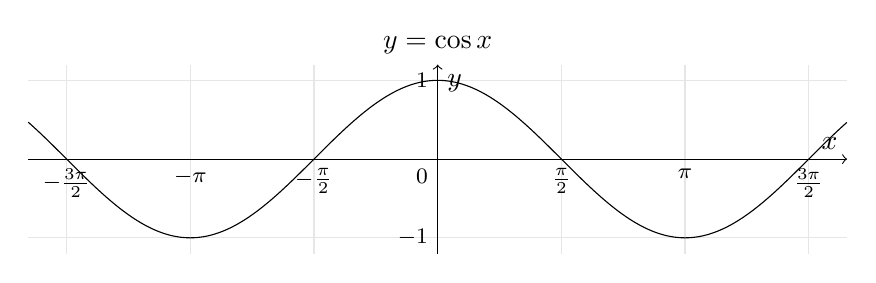
\begin{tikzpicture} \draw[color=gray,opacity=0.2] (-5.2,-1.2) grid[xstep=pi/2](5.2,1.2); \draw[->] (-5.2, 0) -- (5.2, 0) node[above left]{$x$}; \draw[->] (0,-1.2) -- (0, 1.2) node[below right]{$y$}; \foreach \y in {-1} \draw(0,\y) node[left]{\footnotesize$\y$}; \foreach \y in {1} \draw(0,\y) node[left]{\footnotesize$\y$}; \foreach \x[count=\cnt] in {-\frac{\pi}{2},-\pi,-\frac{3\pi}{2}} \draw({(-\cnt/2)*pi},0) node[below]{\footnotesize$\x$}; \foreach \x[count=\cnt] in {\frac{\pi}{2},\pi,\frac{3\pi}{2}} \draw({(\cnt/2)*pi},0) node[below]{\footnotesize$\x$}; \draw(0,0) node[below left]{\footnotesize$0$}; \draw[domain=-5.2:5.2, samples=1000, smooth, variable=\x, black] plot (\x, {cos(\x r)}); \node[above] at (current bounding box.north) {$y=\cos{x}$};\end{tikzpicture}}{39/84}
\slideq{Courbe représentative de $\ash{x}$}{40/84}
\slider{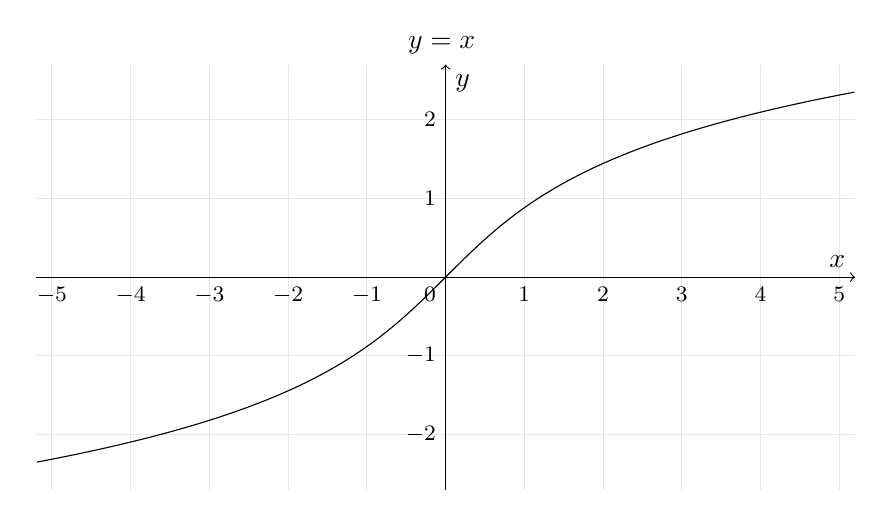
\begin{tikzpicture} \draw[color=gray,opacity=0.2] (-5.2,-2.7) grid (5.2,2.7); \draw[->] (-5.2, 0) -- (5.2, 0) node[above left]{$x$}; \draw[->] (0,-2.7) -- (0, 2.7) node[below right]{$y$}; \foreach \y in {-2,-1,1,2} \draw(0,\y) node[left]{\footnotesize$\y$}; \foreach \x in {-5,...,-1} \draw(\x,0) node[below]{\footnotesize$\x$}; \foreach \x in {1,...,5} \draw(\x,0) node[below]{\footnotesize$\x$}; \draw(0,0) node[below left]{\footnotesize$0$}; \draw[domain=0:5.2, samples=600, scale=1, smooth, variable=\x, black] plot (\x,{ln(\x+sqrt(\x*\x+1))}); \draw[domain=0:5.2, samples=600, scale=1, smooth, variable=\x, black] plot (-\x,{-ln(\x+sqrt(\x*\x+1))}); \node[above] at (current bounding box.north) {$y=\ash{x}$}; \end{tikzpicture}}{40/84}
\slideq{$\lim{x\to+\infty}{\th{x}}$}{41/84}
\slider{$1$}{41/84}
\slideq{Courbe représentative de $\acos{x}$}{42/84}
\slider{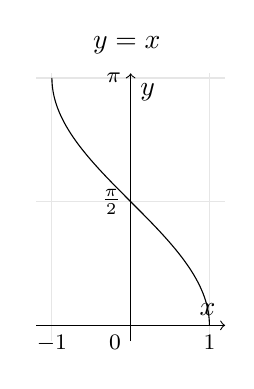
\begin{tikzpicture} \draw[color=gray,opacity=0.2] (-1.2,-0.2) grid[ystep=pi/2](1.2,3.2); \draw[->] (-1.2, 0) -- (1.2, 0) node[above left]{$x$}; \draw[->] (0,-0.2) -- (0, 3.2) node[below right]{$y$}; \foreach \y[count=\cnt] in {\frac{\pi}{2},\pi} \draw(0,{(\cnt/2)*pi}) node[left]{\footnotesize$\y$}; \foreach \x in {-1} \draw(\x,0) node[below]{\footnotesize$\x$}; \foreach \x in {1} \draw(\x,0) node[below]{\footnotesize$\x$}; \draw(0,0) node[below left]{\footnotesize$0$}; \draw[domain=pi:0, samples=400, scale=1, smooth, variable=\x, black] plot ({cos(\x r)},\x); \node[above] at (current bounding box.north) {$y=\acos{x}$}; \end{tikzpicture}}{42/84}
\slideq{$2\cos{\frac{x+y}{2}}\cos{\frac{x-y}{2}}$}{43/84}
\slider{$\cos{x}+\cos{y}$}{43/84}
\slideq{$\sin{x}$\linebreak\linebreak$t=\tan{\frac{x}{2}}$}{44/84}
\slider{$\frac{2t}{1+t^2}$\linebreak\linebreak$t=\tan{\frac{x}{2}}$}{44/84}
\slideq{$\cos{\pi-x}$}{45/84}
\slider{$-\cos{x}$}{45/84}
\slideq{$\sin{\frac{\pi}{2}-x}$}{46/84}
\slider{$\cos{x}$}{46/84}
\slideq{$\der{\ash{x}}$}{47/84}
\slider{$\frac{1}{\sqrt{x^2+1}}$}{47/84}
\slideq{Expression de $\ath{x}$}{48/84}
\slider{$\frac{1}{2}\ln{\frac{1+x}{1-x}}=\ln{\sqrt{\frac{1+x}{1-x}}}$}{48/84}
\slideq{$\lim{x\to-\infty}{\th{x}}$}{49/84}
\slider{$-1$}{49/84}
\slideq{$\cos{x+\pi}$}{50/84}
\slider{$-\cos{x}$}{50/84}
\slideq{$\cos{x+\frac{\pi}{2}}$}{51/84}
\slider{$-\sin{x}$}{51/84}
\slideq{Courbe représentative de $\tan{x}$}{52/84}
\slider{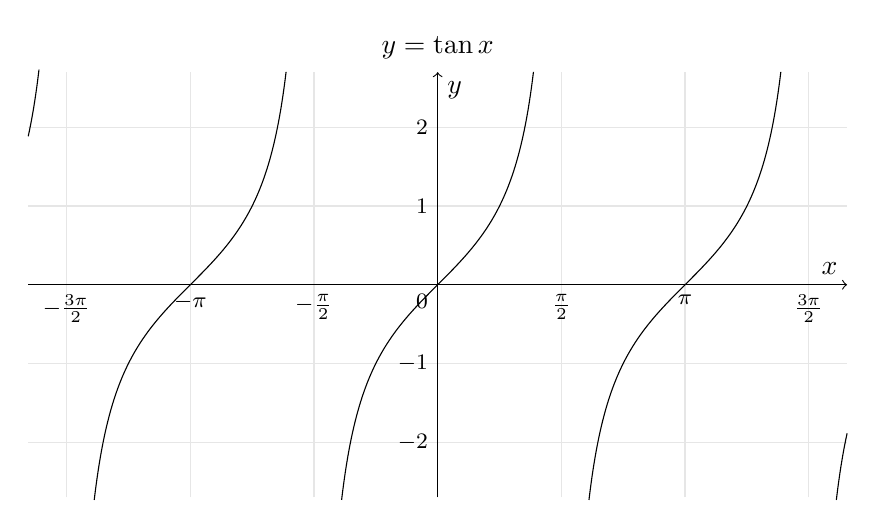
\begin{tikzpicture} \draw[color=gray,opacity=0.2] (-5.2,-2.7) grid[xstep=pi/2](5.2,2.7); \draw[->] (-5.2, 0) -- (5.2, 0) node[above left]{$x$}; \draw[->] (0,-2.7) -- (0, 2.7) node[below right]{$y$};  \foreach \y in {-2,-1} \draw(0,\y) node[left]{\footnotesize$\y$}; \foreach \y in {1,2} \draw(0,\y) node[left]{\footnotesize$\y$}; \foreach \x[count=\cnt] in {-\frac{\pi}{2},-\pi,-\frac{3\pi}{2}} \draw({(-\cnt/2)*pi},0) node[below]{\footnotesize$\x$}; \foreach \x[count=\cnt] in {\frac{\pi}{2},\pi,\frac{3\pi}{2}} \draw({(\cnt/2)*pi},0) node[below]{\footnotesize$\x$}; \draw(0,0) node[below left]{\footnotesize$0$}; \foreach \x in {-1,0,1} \draw[domain=\x*pi-1.22:\x*pi+1.22, samples=500, scale=1, smooth, variable=\x, black] plot (\x,{tan(\x r)}); \draw[domain=-5.2:-2*pi+1.22, samples=500, scale=1, smooth, variable=\x, black] plot (\x,{tan(\x r)}); \draw[domain=2*pi-1.22:5.2, samples=500, scale=1, smooth, variable=\x, black] plot (\x,{tan(\x r)}); \node[above] at (current bounding box.north) {$y=\tan{x}$}; \end{tikzpicture} }{52/84}
\slideq{Courbe représentative de $\th{x}$}{53/84}
\slider{\begin{tikzpicture} \draw[color=gray,opacity=0.2] (-5.2,-1.2) grid (5.2,1.2); \draw[->] (-5.2, 0) -- (5.2, 0) node[above left]{$x$}; \draw[->] (0,-1.2) -- (0, 1.2) node[below right]{$y$}; \foreach \y in {-1,1} \draw(0,\y) node[left]{\footnotesize$\y$}; \foreach \x in {-5,...,-1} \draw(\x,0) node[below]{\footnotesize$\x$}; \foreach \x in {1,...,5} \draw(\x,0) node[below]{\footnotesize$\x$}; \draw(0,0) node[below left]{\footnotesize$0$}; \draw[domain=-5.2:5.2, samples=1100, scale=1, smooth, variable=\x, black] plot (\x,{(exp(\x)-exp(-\x))/(exp(\x)+exp(-\x))}); \node[above] at (current bounding box.north) {$y=\th{x}$}; \end{tikzpicture}}{53/84}
\slideq{$n\in\N^*$, $x\in\R$\linebreak$\der[n]{\ch{x}}$}{54/84}
\slider{$\left\{\begin{matrix*}[l]\ch{x}&\;\text{si }n\in2\N\\\sh{x}&\;\text{sinon}\end{matrix*}\right.\!$}{54/84}
\slideq{$\lim{x\to0}{\frac{\th{x}}{x}}$}{55/84}
\slider{$1$}{55/84}
\slideq{$\tan{2x}$}{56/84}
\slider{$\frac{2\tan{x}}{1-\tan[2]{x}}$}{56/84}
\slideq{$\der{\tan{x}}$}{57/84}
\slider{$\frac{1}{\cos[2]{x}}=1+\tan[2]{x}$}{57/84}
\slideq{$\sin{x}\cos{y}$}{58/84}
\slider{$\frac{1}{2}\l\sin{x+y}+\sin{x-y}\r$}{58/84}
\slideq{$\der{\atan{x}}$}{59/84}
\slider{$\frac{1}{1+x^2}$}{59/84}
\slideq{Argument d'un nombre complexe $z$ avec $\atan{x}$}{60/84}
\slider{$\arg\l z\r\equiv\atan{\frac{\Im\l z\r}{\Re\l z\r}}\,\left[\pi\right]$}{60/84}
\slideq{$\frac{\tan{x}-\tan{y}}{1+\tan{x}\tan{y}}$}{61/84}
\slider{$\tan{x-y}$}{61/84}
\slideq{Valeurs remarquables de $\atan{x}$}{62/84}
\slider{\setcolrow{5}{2}\begin{tikzpicture}[ampersand replacement=\&] \matrix (mat) [table] {  \&$0$\&$\oldfrac{\sqrt{3}}{3}$\&$1$\&$\sqrt{3}$\\ \begin{turn}{45}$\arctan$\end{turn}\&$0$\&$\oldfrac{\pi}{6}$\&$\oldfrac{\pi}{4}$\&$\oldfrac{\pi}{3}$\\}; \draw [line width=0.5mm] (-3*10cm/10,-6.5cm/2) -- (-3*10cm/10,6.5cm/2); \draw [line width=0.5mm] (-10cm/2,0cm) -- (10cm/2,0cm); \draw [line width=0.5mm] (-5cm,-3.25cm) rectangle (5cm,3.25cm); \end{tikzpicture}}{62/84}
\slideq{$\lim{x\to0}{\frac{1-\cos{x}}{x^2}}$}{63/84}
\slider{$\frac{1}{2}$}{63/84}
\slideq{Courbe représentative de $\ch{x}$}{64/84}
\slider{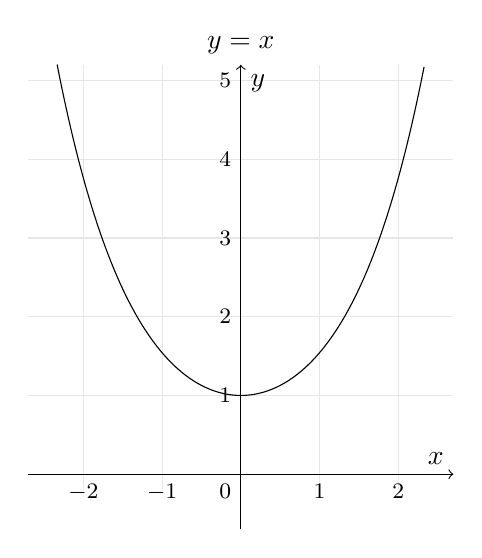
\begin{tikzpicture} \draw[color=gray,opacity=0.2] (-2.7,-0.2) grid (2.7,5.2); \draw[->] (-2.7, 0) -- (2.7, 0) node[above left]{$x$}; \draw[->] (0,-0.7) -- (0, 5.2) node[below right]{$y$}; \foreach \y in {1,...,5} \draw(0,\y) node[left]{\footnotesize$\y$}; \foreach \x in {-2,-1} \draw(\x,0) node[below]{\footnotesize$\x$}; \foreach \x in {1,2} \draw(\x,0) node[below]{\footnotesize$\x$}; \draw(0,0) node[below left]{\footnotesize$0$}; \draw[domain=-2.333:2.333, samples=500, scale=1, smooth, variable=\x, black] plot (\x,{(exp(\x)+exp(-\x))/2}); \node[above] at (current bounding box.north) {$y=\ch{x}$}; \end{tikzpicture}}{64/84}
\slideq{Inégalité classique de $\atan{x}$}{65/84}
\slider{$\forall x\in\R,\;\left|\atan{x}\right|\leqslant\left|x\right|$}{65/84}
\slideq{$-2\sin{\frac{x+y}{2}}\sin{\frac{x-y}{2}}$}{66/84}
\slider{$\cos{x}-\cos{y}$}{66/84}
\slideq{$\sin{x+\frac{\pi}{2}}$}{67/84}
\slider{$\cos{x}$}{67/84}
\slideq{Courbe représentative de $\sh{x}$}{68/84}
\slider{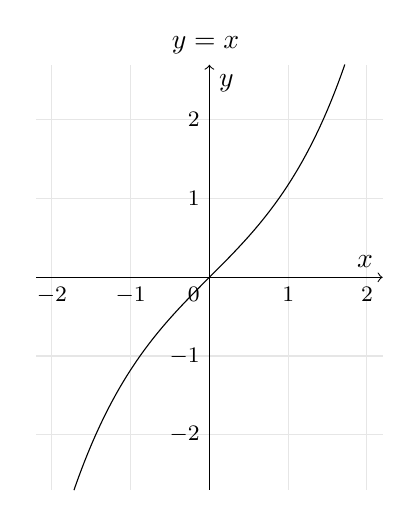
\begin{tikzpicture} \draw[color=gray,opacity=0.2] (-2.2,-2.7) grid (2.2,2.7); \draw[->] (-2.2, 0) -- (2.2, 0) node[above left]{$x$}; \draw[->] (0,-2.7) -- (0, 2.7) node[below right]{$y$}; \foreach \y in {-2,-1,1,2} \draw(0,\y) node[left]{\footnotesize$\y$}; \foreach \x in {-2,-1} \draw(\x,0) node[below]{\footnotesize$\x$}; \foreach \x in {1,2} \draw(\x,0) node[below]{\footnotesize$\x$}; \draw(0,0) node[below left]{\footnotesize$0$}; \draw[domain=-1.72:1.72, samples=400, scale=1, smooth, variable=\x, black] plot (\x,{(exp(\x)-exp(-\x))/2}); \node[above] at (current bounding box.north) {$y=\sh{x}$}; \end{tikzpicture}}{68/84}
\slideq{$\cos{x-y}$}{69/84}
\slider{$\cos{x}\cos{y}+\sin{x}\sin{y}$}{69/84}
\slideq{Propriété remarquable de $\acos{x}$ et $\asin{x}$}{70/84}
\slider{$\acos{x}+\asin{x}=\frac{\pi}{2}$}{70/84}
\slideq{Inégalités classiques de $\sin{x}$}{71/84}
\slider{$\forall x\in\R_+,\;\sin{x}\leqslant x$\linebreak$\forall x\in\R_-,\;\sin{x}\geqslant x$\linebreak$\forall x\in\R,\;\left|\sin{x}\right|\leqslant\left|x\right|$\linebreak$\forall x\in\left[0,\oldfrac{\pi}{2}\right],\;\sin{x}\geqslant\oldfrac{2x}{\pi}$}{71/84}
\slideq{$\cos{x+y}$}{72/84}
\slider{$\cos{x}\cos{y}-\sin{x}\sin{y}$}{72/84}
\slideq{$\frac{1-t^2}{1+t^2}$\linebreak\linebreak$t=\tan{\frac{x}{2}}$}{73/84}
\slider{$\cos{x}$\linebreak\linebreak$t=\tan{\frac{x}{2}}$}{73/84}
\slideq{$\cos[2]{x}-\sin[2]{x}=2\cos[2]{x}-1=1-2\sin[2]{x}$}{74/84}
\slider{$\cos{2x}$}{74/84}
\slideq{Propriétés remarquables de $\asin{x}$}{75/84}
\slider{$\forall x\in\left[-1,1\right],\;\sin{\asin{x}}=x$\linebreak$\forall x\in\left[-\oldfrac{\pi}{2},\oldfrac{\pi}{2}\right],\;\asin{\sin{x}}=x$\linebreak$\forall x\in\left[\oldfrac{\pi}{2},\oldfrac{3\pi}{2}\right],\;\asin{\sin{x}}=\pi-x$}{75/84}
\slideq{$n\in\N^*$, $x\in\R$\linebreak$\der[n]{\sin{x}}$}{76/84}
\slider{$\sin{x+\frac{n\pi}{2}}=\left\{\begin{matrix*}[l]\l-1\r^{\left\lfloor\oldfrac{n}{2}\right\rfloor}\sin{x}&\;\text{si }n\in2\N\\\l-1\r^{\left\lfloor\oldfrac{n}{2}\right\rfloor}\cos{x}&\;\text{sinon}\end{matrix*}\right.\!$}{76/84}
\slideq{$\cos{\frac{\pi}{2}-x}$}{77/84}
\slider{$\sin{x}$}{77/84}
\slideq{$2\sin{\frac{x+y}{2}}\cos{\frac{x-y}{2}}$}{78/84}
\slider{$\sin{x}+\sin{y}$}{78/84}
\slideq{$\frac{1}{2}\l\cos{x+y}+\cos{x-y}\r$}{79/84}
\slider{$\cos{x}\cos{y}$}{79/84}
\slideq{Expression de $\ash{x}$}{80/84}
\slider{$\ln{x+\sqrt{x^2+1}}$}{80/84}
\slideq{$\der{\asin{x}}$}{81/84}
\slider{$\frac{1}{\sqrt{1-x^2}}$}{81/84}
\slideq{$\frac{1}{2}\l\sin{x+y}-\sin{x-y}\r$}{82/84}
\slider{$\cos{x}\sin{y}$}{82/84}
\slideq{$\sin{x}-\sin{y}$}{83/84}
\slider{$2\cos{\frac{x+y}{2}}\sin{\frac{x-y}{2}}$}{83/84}
\slideq{Valeurs remarquables}{84/84}
\slider{\setcolrow{6}{5}\begin{tikzpicture}[ampersand replacement=\&] \matrix (mat) [table] { \&$0$\&$\oldfrac{\pi}{6}$\&$\oldfrac{\pi}{4}$\&$\oldfrac{\pi}{3}$\&$\oldfrac{\pi}{2}$ \\ $\oldsin$\&$0$\&$\oldfrac{1}{2}$\&$\oldfrac{\sqrt{2}}{2}$\&$\oldfrac{\sqrt{3}}{2}$\&$1$\\ $\oldcos$\&$1$\&$\oldfrac{\sqrt{3}}{2}$\&$\oldfrac{\sqrt{2}}{2}$\&$\oldfrac{1}{2}$\&$0$\\ $\oldtan$\&$0$\&$\oldfrac{1}{\sqrt{3}}$\&$1$\&$\sqrt{3}$\&--\\ $\oldcot$\&--\&$\sqrt{3}$\&$1$\&$\oldfrac{1}{\sqrt{3}}$\&$0$\\ }; \draw [line width=0.5mm] (-10cm/3,-6.5cm/2) -- (-10cm/3,6.5cm/2); \draw [line width=0.5mm] (-10cm/2,3*6.5cm/10) -- (10cm/2,3*6.5cm/10); \draw [line width=0.5mm] (-5cm,-3.25cm) rectangle (5cm,3.25cm);\end{tikzpicture}}{84/84}
\end{document}